\vspace*{-0.3cm}
\section{Related Work}
\label{section:related-work}

\costas{add plotly and Bokeh}

The specific template language used in our project, follows heavily the syntax of templates in the FORWARD project \cite{SIGMOD2010,CIDR2011}. However, the semantics are different in order to fit the needs of notebook operation. Namely, the templates operate as scripts that produce nested Python instances for the units and fully redisplay them in each round. Unlike FORWARD, it is predetermined which units will be shown on each snapshot of the notebook. Thus, at the present state, it is not yet possible to create an interface that is tantamount to, say, a data cube exploration - which is something that would be possible in FORWARD. On the positive side, ViDeTTe (unlike FORWARD) does not require the analyst to understand the notebook as an MVVM application, whereas in each snapshot the framework visualizes a page with potentially different units and/or partially modified unit instances. 

Additional prior work related to \projname\ notebooks can be classified into the following categories:
\eat{
{\bf MVVM frameworks.} The idea of allowing application developers to use a declarative language to develop a web application has been the main selling point of many recent application frameworks, such as \angular\ \cite{angularjs}, \react\ \cite{react}, Ember \cite{ember} and others \cite{knockout, catel, mvvmcross, mvvmlight}.  These frameworks follow the MVVM (Model-View-ViewModel) paradigm, according to which a declarative template transforms a logical description of the data (referred to as \emph{model}) to a logical description of the visual state (also known as \emph{viewmodel}), which is then rendered as a visual page instance (also known as \emph{view}). Similarly to \projname, the declarative nature of the template increases developer productivity by simplifying the application specification \costas{development?} and automating the change propagation. However, as has been the case with many early declarative frameworks that automate tasks that were previously dealt with imperative code, existing MVVM frameworks still exhibit important inefficiencies. In particular, their change propagation algorithms are extremely inefficient, with a complexity that depends on the size of the entire model (i.e., the data) and/or the viewmodel (i.e., the template instance), instead of depending only on the number of the changes in the model and in the viewmodel, as is the case in \projname. Moreover, they either do not support JavaScript visualization libraries (as is the case with \react\ \cite{react}) or when they do (as is the case with \angular\ \cite{angularjs}) the process of wrapping existing libraries is very laborious. Finally, they limit the expressiveness of their template languages due to limitations of their change propagation algorithms. For a detailed comparison of \projname\ to MVVM frameworks, the reader is referred to Section \ref{section:angular-vs-forward}.

{\bf Incremental view maintenance approaches.} The concept of change propagation has been extensively studied in the database community in the form of incremental view maintenance (IVM). This has led to a substantial number of works both older  \cite{vm-blt-86, vm-bcl-89, vm-91, vm-qw-91, view-sigmod-93} and more recent \cite{dbtoaster-vldbj-2014, idivm-sigmod-2015} (see \cite{survey-deb-95,mv-survey-12} for surveys of IVM works). While inspired from IVM techniques, our change propagation algorithm extends existing IVM techniques in several important directions: it extends both the supported data model (adding support for semi-structured data and ordered collections) and the expressivity of the query language (adding support for user defined functions). Moreover, in contrast to IVM approaches which do not have any restrictions on the type of output diffs that they create, \projname's propagation algorithm has to respect the capabilities of the units (expressed in the form of supported unit instance diffs). For a detailed discussion of IVM works and their relationship to \projname, the reader is referred to Section \ref{section:ivm-discussion}.

{\bf Dynamic algorithms.} Change propagation has also been studied in the algorithms community in the form of dynamic algorithms. A dynamic algorithm efficiently updates the result of a computation, such as a clustering algorithm \cite{datta1993static}, a computational geometry algorithm \cite{chiang1992dynamic} or an algorithm that generates shortest path trees \cite{frigioni2000fully}. Although dynamic algorithms have been successfully used in many domains, they are tailored to a particular computation and cannot be easily extended to other classes of computations.

{\bf Incremental computation.} Change propagation has also been studied in the programming language community under the title of incremental computation. \yannisk{I am not sure yet what to say about these approaches. To get some background please see the commented out text by Costas and the corresponding wikipedia page on `incremental computing'}
}


%We mentioned the most closely related work, namely MVVM frameworks, in the previous sections of the paper. In section \ref{sec:mvvm-change-propagation}, we describe the fundamental limitations that prohibit such frameworks from operating in an efficient manner. Additionally, in section \ref{sec:ivm-in-databases} we describe the main focus of IVM techniques employed by database systems which is what powers our propagation algorithms. In this section, we briefly describe work that is more peripherally related to the concept of change propagation. This work has been conducted by researchers mainly in the fields of programming languages and algorithms.

%In the algorithms community, researchers have worked on designing dynamic algorithms that are capable of efficiently updating their output given dynamic changes on their input. Surveys that have been conducted in this area \cite{chiang1992dynamic} describe numerous approaches that have offered significant speedups in functions that resolve individual computational problems, especially when such functions operate on big data. These surveys also describe the significant effort that is usually associated with the development and implementation of such algorithms. Some of these algorithms took years of research to be developed and they are mostly oriented towards solving expensive domain specific problems (such as problems in computational geometry), while many such problems still remain open. Since these algorithms were carefully designed for solving individual computational problems they are not extensible in a way that would allow them to solve a wider range of problems. For that reason, they are cannot be used to perform change propagation in applications, mainly due to the diversity that such applications exhibit. 
 
%Elixir is a dynamic, functional language designed for building applications. Ecto is a domain specific language (Object-Relational mapping - ORM) that can be used in conjuction with Elixir to enable interaction with databases. One of the key concepts of Ecto (and other ORM libraries (such as doctrine, hibernate) is the notion of changesets. A Changeset -in this context- is essentially a construct that includes all the changes that will be applied to a back-end database as a result of user interaction. Ecto's API can be used to perform filtering, validation or describe extra constraints to a changeset before that is applied to a database. While this a fairly useful feature that assists in staging modifications and can potentially completely avoid or limit unnecessary or erroneous interactions with back-end databases by pushing down constraints to the application level, it cannot be used to efficiently propagate changes from the databases to the view (or the other way). Therefore, while both these tools and \projname utilize sets of changes their ultimate purpose is very different. 
 
%Meteor is a development platform that combines third party client-side libraries (such as AngularJS, ReactJS, Blaze, Cordova and others) and server-side libraries and databases (such as NodeJS, Connect, MongoDB and others) to enable the relatively effortless development of full-stack applications. While developer-friendliness of full stack applications is also one of the goals of \projname\, in \projname\ this is accomplished by using novel components that were designed from scratch with power and memory efficiency as a main priority. Meteor on the other hand, simply reuses existing software solutions across the stack.

%The goal of ZQL, which is the query language of Zenvisage, is to enable data analysts to extract visualizations that assist in identifying trends, patterns and insights from various sources in a declarative fashion. While ZQL manages to query databases and construct visualizations using minimal lines of code, the syntax of ZQL is more oriented towards data exploration experts therefore it is not very user friendly for application developers. Additionally, Zenvisage does not support unit wrapping, for that reason the user is limited to only utilizing a predefined set of available visualizations. Lastly, even if the underlying data used to construct a visualization change, Zenvisage will not automatically reflect those changes to the visualization (incrementally or otherwise). Instead the user has to reissue the ZQL query in order to reconstruct the update visualization.  

%In the programming languages community, researchers have developed techniques that achieve automatic incrementalization of programs. The main focus of these techniques \cite{ramalingam1993categorized} is the automatic translation of conventional programs into respective programs that can respond to dynamically changed data. Since these techniques provide tools or compiler techniques that automatically perform this translation, they manage to minimize the effort required for the implementation of such functions. Recent work on self adjusting computations also includes the use of specially designed high level languages (or the extension of existing languages with annotations \cite{hammer2009ceal, chen2012type}) used to express incremental computations that when combined with specifically developed compilers, can generate executables capable of efficiently handling mutations of input data. 

%A common denominator of the majority of these techniques is the fact that the underlying languages utilize a strong type system that enables the automatic distinction, (or in many cases the explicit manual distinction) between mutable and immutable input data. Leaving aside the fact that applications developers cannot necessarily predict which input data will be modified during the lifetime of an application, the fact that JavaScript is an untyped language can also be an obstacle, in using such techniques. It is unclear if these techniques could be used without forcefully introducing a type-system that application developers would have to adapt to. While, such a type-system might potentially assist in using some of these techniques to power incrementally maintained web applications, it would also steepen the learning curve of the respective framework since developers would have to familiarize themselves with the new type system. Lastly, it is unclear how such techniques can be used in a distributed architecture like the one described in Section \ref{sec:ivm-general}


\eat{
{\bf Declarative data-driven visualizations.} Finally, recent works in data-driven visualizations have suggested the use of declarative languages for the specification of visualizations. Notable examples of such works include Vega \cite{???} \yannisk{Is it Vega or Vega-lite?} and Zenvisage \cite{???}. While these works share the same observation with the current work that declarative languages can simplify the visualization specification process, they use declarative languages to accomplish different goals. Zenvisage's language is tuned towards easy data exploration, by allowing the user to create visualizations that reveal interesting patterns in the data. Vega... \yannisk{Costa, please add citations above and text on Vega}. In contrast, \projname\ leverages the declarative language to allow the specification of fully-fledged web applications that can use any of the existing JavaScript visualization libraries.
}

{\bf Grammar-based visualizations.} The concept of using a formal grammar to specify visualizations can be traced back to Wilkinson's ``The Grammar of Graphics" \cite{Wilkinson:2005:GG:1088896}. Since then multiple tools, such as Polaris \cite{stolte2002polaris} (later commercialized as Tableau), ggplot2 \cite{wickham2009ggplot2}, Vega \cite{satyanarayan2015vega, vega} and others \cite{ggvis, bostock2009protovis, d3} have adopted this approach, thus enabling the description of visualizations (as well as the user interaction with such visualizations \cite{Wu:2016:DAI:2939502.2939517, satyanarayan2016reactive}) in a terse and declarative manner. While the expressiveness of the employed grammars varies, their main focus is to effectively describe the specifics of the visualizations that will appear (for instance the dimensions of the chart, the colors, etc.), and not to describe data access or data processing and/or conversions. For that reason, such tools do not provide constructs capable of retrieving data from various sources or performing data transformations. Instead, the user has to manually perform these tasks and convert the dataset she wants to visualize into the format that is expected by the respective tool in order to generate the visualization.


\eat{
allow users to access data from various sources and most importantly they do not provide any data conversion modules capable of transforming the data to the required data type for the visualization. Therefore, the user has to manually convert the dataset she wants to visualize into a format that matches the expected schema and then simply evaluate it to generate the respective chart. 
}
{\bf Data exploration.}  Tools that use the human factor as an integral part of data exploration have gained in popularity in the past years. Such tools provide a simple to use way that describes both computation and visualizations, thus providing the required toolkit to effectively explore data and steer computation. Some of these tools enable this process by providing a declarative language capable of performing such tasks (such as Zenvisage \cite{DBLP:journals/corr/SiddiquiKLKP16} and Devise \cite{livny1997devise}), while others (such as Vizdom \cite{crotty2015vizdom}, DataHub \cite{Krishnan:2016:AID:2994509.2994514} and more\cite{derthick1997interactive,  bhardwaj2015collaborative, zoumpatianos2015rinse, DBLP:conf/icde/LiarouI14, Kamat:2016:TSI:2939502.2939514}) rely on the user interaction with a front-end, in order to compose the appropriate queries. As a result, the former tools assume a type of user with deep understanding in databases and query languages, while the latter offer a more user-friendly way of performing an analysis \eat{pertaining to a user that does not have to have such a strong background in the field }but at the same time allow a predetermined set of possible analyses. \projname\ notebooks bridge the gap between these two types of users; to a data analyst it provides constructs that allow rapid creation of notebooks for an arbitrary number of analyses, while to a non-technical user it provides the capability to interact with the produced visualization in order to further explore the underlying data.


%The goal of ZQL, which is the query language of Zenvisage, is to enable data analysts to extract visualizations that assist in identifying trends, patterns and insights from various sources in a declarative fashion. While ZQL manages to query databases and construct visualizations using minimal lines of code, the syntax of ZQL is more oriented towards data exploration experts therefore it is not very user friendly for application developers. Additionally, Zenvisage does not support unit wrapping, for that reason the user is limited to only utilizing a predefined set of available visualizations. Lastly, even if the underlying data used to construct a visualization change, Zenvisage will not automatically reflect those changes to the visualization (incrementally or otherwise). Instead the user has to reissue the ZQL query in order to reconstruct the update visualization.  



\eat{
\subsection{AngularJS}

Perhaps the most widely used MVVM web framework currently is AngularJS \cite{angularjs}. Angular is mainly supported and maintained by Google, but since it's an open source framework \cite{angularjsopensource} it also has a very rich community of contributors, which ranges from individuals to big corporations. From the perspective of the application developer AngularJS requires very little boilerplate code for most simple applications. Particularly the developer's only responsibility is to specify the Model of the application and create the bindings between the Model and the View by utilizing the template language. When the state of the application is modified Angular is able to infer how the respective view will be affected, and it will automatically apply the appropriate changes to it.


\begin{figure}[t]
\begin{code}
 /* ... Additional logic ... */
 $http.get('http://forward.ucsd.edu/delivery_truck_service')
 .then(function(result) \{
    $scope.delivery\_trucks = result.data;
 \});
 /* ... */
\end{code}
\caption{Part of the Controller used in running example }
\label{figure:angular-controller-snippet}
\end{figure}




\begin{figure}[t]
\begin{code}
<html>
   <!-- ... imports and other irrelevant 
            parts of the template ... -->
   <div ng-app="truck\_delivery" ng-controller="delivery\_ctrl">
     <!-- ... other HTML tags ... -->
     <div id="map\_container">
      <ui-gmap-google-map 
      center="map.center" zoom="map.zoom" bounds="map.bounds">
        <ui-gmap-marker ng-repeat="truck in delivery\_trucks" 
        idKey="truck.truck\_key"
        coords="truck.coords">
        </ui-gmap-marker>
       </ui-gmap-google-map>
     </div>
   </div>
   <div>
     <table>
       <tr> <!-- ... column labels ... --> </tr>
       <tr ng-repeat="truck in delivery\_trucks">
            <td> \{\{truck.VIN\}\} /td>
            <td> \{\{truck.driver\}\} /td>
            <td> \{\{truck.shift_start_time\}\} /td>
            <td> \{\{truck.avg_speed\}\} /td>
            <td> 
              <progressbar type="Circle" 
              strokeWidth="10" trailWidth= "1"
              easing= "easeInOut" fromColor="#FC5B3F"
              fromWidth="1" toColor="#6FD57F" toWidth="10"
              numerator = "truck.delivered_items" 
              denominator="truck.total_items"
              ></progressbar>
            </td>
       </tr>
     </table>
   </div>
    <!-- ... rest of template ... -->
</html>
\end{code}
\caption{Angular Template \texttt{Delivery-Trucks}}
\label{figure:angular-template-language}
\end{figure}


Angular's template language consists of HTML tags that may contain additional Angular specific attributes which are utilized for binding data to the corresponding parts of the View. Other than HTML, the template language can also contain custom tags that instantiate reusable units, namely Angular Directives; \textbf{Angular Directives} are modules that wrap existing JavaScript visual layer components such as Google Maps\cite{gmaps}, HighCharts\cite{kuan2012learning} and more, in a way that favors re-usability and code minimalism. When importing such directives the application developer is able specify the state of the visual layer using declarative logic. This greatly reduces the imperative code that has to be written and maintained, since the developer is no longer responsible for explicitly implementing code that reflects every potential modification of the Model. The Model of the application however is specified by using JavaScript code which, despite the fact that it may contain functional expressions, it still is mostly imperative. In order for a variable $v$ to be used within Angular's template language the application developer has to utilize a Controller to instantiate the contents of the afore-mentioned variable and then attach it to the $scope$ object; the  scope object is a crucial part of AngularJS internal architecture as we will describe later in this section. The contents of the variables that the application devleoper attaches to the scope are Plain Old JavaScript Objects (POJO). Lastly, Angular provides two more tool-sets, namely Services and Factories, that mostly assist in data transfer used for the instantiation or update of the Model. These modules can be used to write and read data to and from local or remote databases or web-services

\eat{
. These modules mostly assist in data transfer to and from back-end web-services, local and remote databases and since the classes that describes them is extensible it enables further code reusability within an application.
}
In Figures \ref{figure:angular-controller-snippet} and \ref{figure:angular-template-language} we show a part of the controller and the template language that is used to generate the running example shown in Figure \ref{figure:running-example:deliverymap-screenshot}. In Figure \ref{figure:angular-controller-snippet} we showcase a small snippet that utilizes the http service to perform an asynchronous HTTP GET request to a remote server, retrieve the result and attach it to the scope variable, under the attribute name $delivery\_trucks$. In Figure \ref{figure:angular-template-language} we show a snippet of the template that generates the majority of the view of the running example. In line 4 on the template we specify the AngularJS application name and the corresponding controller name of the angular application by utilizing the ng-app and ng-controller attributes. In lines 7-13 we use a Google Maps custom directive to generate the map shown in Figure \ref{figure:running-example:deliverymap-screenshot}, in lines 25-31 we use a ProgressBar directive that manages the progress bars that appear in the HTML table. Notice that in these two cases we use special attribute names to create a binding between some parts of the model (for instance, the coords of the delivery trucks) and the View (for instance the coordinates of the respective marker). In lines 9 and 19, ng-repeat iterates over the entire delivery\_trucks array and at each iteration it initializes an alias for each truck, additionally it replicates the current directive and every child directive $n$ times, with $n$ being the total number of elements the $delivery\_trucks$ contains. 






\textbf{Angular's Watchers - Dirty Checking}

Every time the application developer binds a single variable or expression to the template, Angular attaches a watcher to the scope object. Watchers are essentially trigger definitions that execute when a mutation occurs on the part of the model that is being watched. A watcher contains the expression that is being watched, namely: WatchExpression, the Listener and the objectEquality variable. The WatchExpression can be anything from a function call, to a reference to a part of the Model. When the current result of the WatchExpression changes Angular triggers the Listener, which is a callback function that is responsible for updating the respective part of the view. In order for the framework to decide if the result of the WatchExpression changed it needs to compare the current state of the returned object with the previous state, this process is called dirty-checking. The kind of comparison that will take place is defined by the objectEquality, in general two types of comparisons are allowed: deep and shallow; in a shallow comparison, Angular will trigger the Listener function when the WatchExpression returns a completely new object (The reference to the watched object changes), while in a deep comparison Angular will iterate over all the children of the currently returned object and it will trigger the Listener function if one of these nodes is different from the respective node of the previous returned object. In order to perform dirty-checking, Angular needs to store both the pre-state and the current state of the returned object, therefore the memory and the processing footprint will be higher, the bigger the watched object is.

\textbf{The Digest Cycle}

A crucial part of the internal architecture of Angular is the Digest Cycle. This algorithm in collaboration with the dirty-checking that is performed for each watcher is responsible for propagating to the View changes that occur on the Model. The digest cycle is initiated when an event triggers an action that is part of the Angular scope. During this process, Angular iterates over all the watchers that exist in the scope and it compares the old result (pre-state) of the WatchExpression with the current one, if a difference is found then the corresponding Listener function is triggered. If some Listener function modifies the Model then the digest cycle will get initiated once again; this iteration will continue until either the Model stabilizes or the digest cycle executes 10 times, after which Angular throws an exception and the Angular application is killed. As we observe the complexity of the digest cycle is proportional to the total numbers of watchers that have been declared, additionally if deep watchers are used then the complexity becomes even worse since for each deep watcher the entire watched object will have to be traversed so that nested values will be inspected for changes. If $w$ is the number of watchers that have been declared and $o$ is the size of watched object, with $o$ being equal to 1 in the case of shallow watches, then the algorithm that performs updates to the view given changes on the model is $O(wd)$.

\eat{
This is a very similar concept to the action-page cycle that we describe in section \ref{section:web1.0} (shown in Figure \ref{figure:action-page-cycle}). As the user interacts with the view or new data are coming from the server, events trigger actions. Each of these actions eventually, initiate the digest-cycle. During this process, Angular iterates over all the watchers that exist in the scope object and it compares the old WatchExpression with the new one, if a difference is found then the corresponding Listener function is triggered. If the callback function modifies the Model then the digest cycle will get initiated once again, this will continue until either the Model stabilizes or until the digest cycle executes 7 times.
}




\eat{

\begin{figure}
\begin{code}
\directive{template}{delivery-trucks (product_name)}
 \directive{import}{functions}
 \directive{import}{actions}

 \textbf{<\% refresh} delivery_trucks =
     SELECT latitude, longitude, VIN, driver, 
            shift_start_time, avg_speed, 
            delivered_items, total_items
     FROM   delivery_trucks_table dtt, 
            product_delivery_truck_relation r, 
            products p
     WHERE  p.name = \directive{print}{product_name} 
            AND dtt.id = r.t_id AND p.id = r.p_id
 \textbf{\%>}
 \directive{html}{}
   <div>
     \directive{unit}{Google-Maps}
     \{
       options : \{
         zoom: 10,
         center: \{
           lat: -25.363882,
           lng : 131.044922
         \},
       \},
       markers : [ 
         \directive{for}{truck \textbf{in} delivery_trucks}
         \{
           position : \{
             lat : \directive{print}{truck.latitude},
             lng : \directive{print}{truck.longitude}
           \}      
         \}
       ]
     \}
     \directive{end unit}{}
   </div>
   <div>
     <table>
       <tr> <!-- ... column labels ... --> </tr>
       \directive{for}{truck \textbf{in} delivery-trucks}
          <tr>
            <td> \directive{print}{truck.VIN} /td>
            <td> \directive{print}{truck.driver} /td>
            <td> \directive{print}{truck.shift_start_time} /td>
            <td> \directive{print}{truck.avg_speed} /td>
            <td> 
               \directive{unit}{ProgressBar} 
               \{
                 type = 'Circle',
                 strokeWidth: 10,
                 trailWidth: 1,
                 easing: 'easeInOut',
                 from: \{ color: '#FC5B3F', width: 1 \},
                 to: \{ color: '#6FD57F', width: 10 \},
                 value : \{
                  numerator :\directive{print}{truck.delivered_items}
                  denominator : \directive{print}{truck.total_items}
                 \}
                \}
                \directive{end unit}{}
            </td>
          </tr>
         \directive{end for}{}
     </table>
   </div>
 \directive{end html}{}
\directive{end template}{}
\end{code}
\caption{Template \texttt{Delivery-Trucks}}
\label{figure:running-example:delivery_trucks-template}
\end{figure}
}

\subsection{EmberJS}

\costas{I have to introduce two-way data binding and perhaps some template languages like moustache etc...}


\begin{figure}[t]
\centering
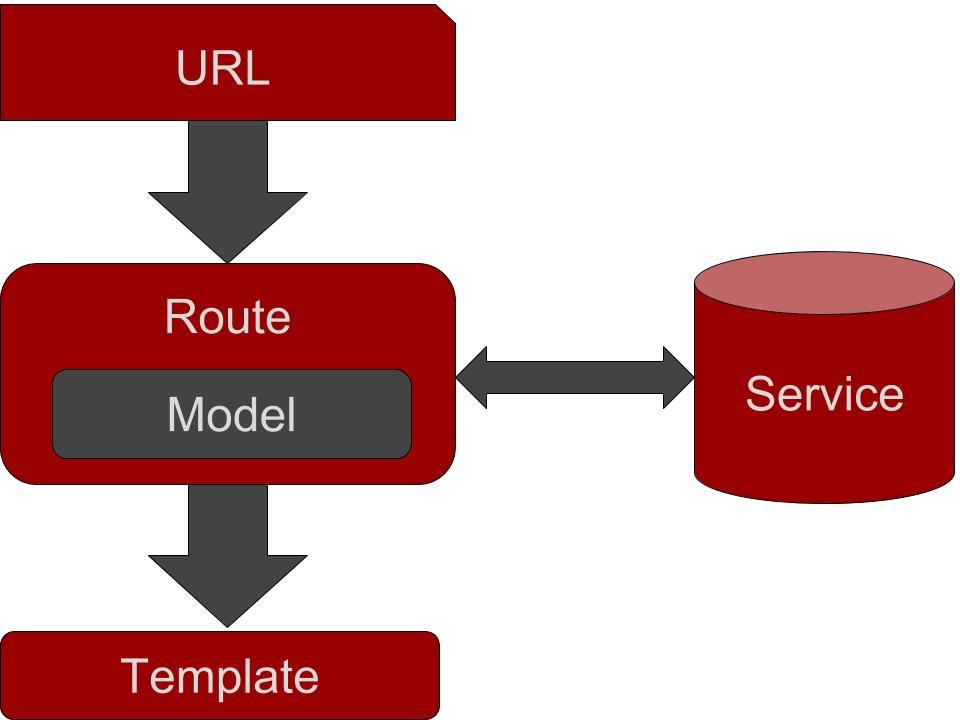
\includegraphics[width=\columnwidth]{figures/ember-programming-model}
\caption{Ember's Programming model}
\label{figure:ember-programming-model}
\end{figure}




Another framework that follows in the footsteps of Angular is EmberJS \cite{ember}. Just like every other MVVM framework, Ember also tries to achieve code minimalism by freeing the application developer from unnecessary boilerplate code and by utilizing declarative code when that seems fit. This framework adopts the action-page programming model, but since it's a client-side framework the entire action-page cycle takes place on the client. Ember's ecosystem comprises Routes, Models, Templates and Services. As shown in Figure \ref{figure:ember-programming-model} Ember's life-cycle starts when the user navigates to a URL that is bound to a particular Route. When the Route receives the event it generates the Model and calls the appropriate renderer that will generate the visual layer of the application. The Route can also utilize the appropriate reusable Services to receive essential data for the construction of the Model (application state).

Ember uses regular expressions to bind a Route to a particular URL. These expressions can also treat parts of the URL as variables, which enables message passing to and from other Routes. As we mentioned earlier Routes are responsible for constructing the Model of the application. Unlike Angular's Model which comprises Plain Old JavaScript Objects, Ember requires the extension of its internal Model objects. This is performed in order to enable efficient message passing between Model objects (as we will mention later), but it has a negative impact on the user friendliness, since the application developer needs to familiarize himself with the internal data structures used by Ember and the respective API that will be used to interact with them, which steepens the learning curve of the framework. Ember Routes are also able to utilize Services whose main goal is to assist in data transfer between local and remote databases and web services (Similar to Angular's Factories and Services).


\eat{
When a particular regular expression matches a URL, the respective Route will construct the Model by accessing a Service. The objective of Services is fairly similar to Angular's Factories and Services, their main goal is to assist in data transfer between local and remote databases and web services. After the appropriate dataset has been received from the Route, it has to construct the Model that is necessary for the next page that will be displayed. Unlike Angular's Model which comprises Plain Old JavaScript Objects, Ember requires the extension of its internal Model objects. This is performed in order to enable efficient message passing between Model objects (as we will mention later), but it has a negative impact on the user friendliness, since the application developer needs to familiarize himself with the internal data structures used by Ember, which steepens the learning curve of the framework.
}

EmberJS does not have its own custom template language, it instead utilizes a third-party template language called, HandlebarsJS \cite{handlebars} to generate the templates. Ember enables component wrapping by providing expendable Components (that are very similar to Angular's Directives). When importing such components the application developer can declaratively pass the Model that will be utilized by the component to generate (or update) the component specific view. Furthermore Ember provides modules that are very similar to Angular's Watchers, namely: Computed properties and Observable classes. These modules are used to listen for changes on the Model and cause the appropriate modifications on the application state. Computed values are mostly used when properties of the Model need to be composed by one or more other basic observable properties. When the computed property is initiated and one of the observable properties are updated, the computed property will be updated as well. Observable classes are mostly used to specify behaviors that will take place when the observable part of the Model changes. The application developer needs to provide a callback function, which most of the times contains imperative logic, in order to specify the respective behavior. 



\textbf{Accessors}

As we mentioned earlier Ember requires the usage of its internal object to represent the Model of the application. Particularly the application developer utilizes getters and setters when he wishes to retrieve and update the value of some Model variable. When the application developer sets a new value to some Model object an event triggers all the respective getters that are associated with that variable and causes them to re-evaluate the returned value. By doing so the application keeps the Model in sync at all times, without wasting resources by iterating over all the watched variables.





\eat{

\begin{figure}
\begin{code}
\directive{template}{delivery-trucks (product_name)}
 \directive{import}{functions}
 \directive{import}{actions}

 \textbf{<\% refresh} delivery_trucks =
     SELECT latitude, longitude, VIN, driver, 
            shift_start_time, avg_speed, 
            delivered_items, total_items
     FROM   delivery_trucks_table dtt, 
            product_delivery_truck_relation r, 
            products p
     WHERE  p.name = \directive{print}{product_name} 
            AND dtt.id = r.t_id AND p.id = r.p_id
 \textbf{\%>}
 \directive{html}{}
   <div>
     \directive{unit}{Google-Maps}
     \{
       options : \{
         zoom: 10,
         center: \{
           lat: -25.363882,
           lng : 131.044922
         \},
       \},
       markers : [ 
         \directive{for}{truck \textbf{in} delivery_trucks}
         \{
           position : \{
             lat : \directive{print}{truck.latitude},
             lng : \directive{print}{truck.longitude}
           \}      
         \}
       ]
     \}
     \directive{end unit}{}
   </div>
   <div>
     <table>
       <tr> <!-- ... column labels ... --> </tr>
       \directive{for}{truck \textbf{in} delivery-trucks}
          <tr>
            <td> \directive{print}{truck.VIN} /td>
            <td> \directive{print}{truck.driver} /td>
            <td> \directive{print}{truck.shift_start_time} /td>
            <td> \directive{print}{truck.avg_speed} /td>
            <td> 
               \directive{unit}{ProgressBar} 
               \{
                 type = 'Circle',
                 strokeWidth: 10,
                 trailWidth: 1,
                 easing: 'easeInOut',
                 from: \{ color: '#FC5B3F', width: 1 \},
                 to: \{ color: '#6FD57F', width: 10 \},
                 value : \{
                  numerator :\directive{print}{truck.delivered_items}
                  denominator : \directive{print}{truck.total_items}
                 \}
                \}
                \directive{end unit}{}
            </td>
          </tr>
         \directive{end for}{}
     </table>
   </div>
 \directive{end html}{}
\directive{end template}{}
\end{code}
\caption{Template \texttt{Delivery-Trucks}}
\label{figure:running-example:delivery_trucks-template}
\end{figure}
}

}

\eat{

\subsection{AngularJS}
\yannisk{This section includes for now a detailed comparison to AngularJS meant for our own understanding of the framework. Once it is ready, we will abstract out the important information and move it to the MVVM framework discussion above and/or to the complexity analysis} \yannisk{Costa, please use the command `projname' instead of `FORWARD' to refer to the framework's name.}

AngularJS (or simply Angular) is an open-source client side web application framework that has gained in popularity over the past few years. Angular is mainly maintained by Google but it has a big community of contributors and it has been used by multiple application developers throughout the globe. A simple search on StackOverflow will return over 120,000 results and a similar search on GitHub will return more than 88,000 repositories that have utilized AngularJS.

Angular's programming model has several similarities to FORWARD's. An AngularJS application is mainly comprised of \textit{Templates}, \textit{functions} and \textit{variables}. Within an AngularJS \textit{Template} the application developer utilizes Angular's template language to specify an abstraction of the view. Angular's template language contains pure HTML along with custom HTML tags and attributes which constitute an extension over the standard HTML directives, these are called Angular Directives. Angular's \textit{templates} just like FORWARD's contain bindings with \textit{variables} and \textit{function}. These bindings act as place-holders. During, run-time the variables and actions get evaluated and linked to the template thus generating a view on the browser. 


When events are triggered in an Angular application, they may cause side effects on the data model (variables and functions). When such changes occur Angular reflects them to the view. A big distinction from FORWARD is the fact that in Angular this happens automatically, there is no concept of manual action-page cycle, therefore the application developer has no controller over when do the changes get reflected to the view. Additionally if there are more than one sub-templates the application developer cannot choose the ones he wants to update, all of them will be updated. This can be extremely inefficient since in modern Angular applications a developer can choose to hide some sub-templates from the view (by using the css property "display:none"), if this is the case and a variable that is bound to several hidden sub-templates changes, angular will proceed to modify all the hidden sub-templates, even though the user will not be able to witness those changes.

\subsubsection{Angular's Digest Cycle}
Even though angular does not have the concept of a manual action-page cycle, it still manages to reflect changes of the model to the visual layer, and the way it accomplishes this with is called \textit{digest cycle}. 

}